\section{Alternative background modeling through calibration}
\label{v5-sec:calibration}\label{sec:v5-calibration}
Calibration asks how the quoted limit would behave if the experiment were
repeated under specified backgrounds. It changes the probability attached
to the likelihood statistic, while retaining the observed counts and the
fitted signal. In this study it is also a way to propagate a finite set of
alternative background shapes through the same analysis. It cannot identify
which shape is the true background.

There are two choices of fit and two choices of probability calculation.
A fixed-background fit treats the estimated mean as known. A profiled fit
allows correlated changes constrained by the GP covariance. Either fit
can use asymptotic formulae or distributions obtained from repeated
experiments. Figure~\ref{v5-fig:calibration-flow} separates these choices.

\begin{figure}[htbp]\centering\small
\fbox{\parbox{0.88\linewidth}{\centering
Choose the frozen support, kernel coordinates, mask, resolution and signal
normalization. Declare the local-GP and archived-stress generating spectra.}}
\\[5pt]$\downarrow$\\[5pt]
\fbox{\parbox{0.88\linewidth}{\centering
Generate complete Poisson spectra at fixed physical signal strengths.
Retrain sideband means and count-dependent errors for every spectrum.
Pass each spectrum to both fits.}}
\\[5pt]$\downarrow$\\[5pt]
\begin{tabular}{cc}
\fbox{\parbox{0.40\linewidth}{\centering\textbf{Profiled background}\\
Fit signal and correlated background nuisance parameters; retain the GP
constraint penalty.}} &
\fbox{\parbox{0.40\linewidth}{\centering\textbf{Fixed background}\\
Fit signal with the retrained GP mean fixed; omit its estimation
uncertainty from the fit.}}\\[5pt]
$\downarrow$ & $\downarrow$\\[5pt]
\fbox{\parbox{0.40\linewidth}{\centering
Build the profiled likelihood-ratio distributions under B and S+B.}} &
\fbox{\parbox{0.40\linewidth}{\centering
Build the fixed-mean likelihood-ratio distributions under B and S+B.}}
\end{tabular}
\\[5pt]$\downarrow$\\[5pt]
\fbox{\parbox{0.88\linewidth}{\centering
For each fit and each truth, invert the empirical $CL_s=0.10$ rule.
Report the larger of the two truth-specific endpoints, with Monte Carlo
precision information. Test the rule on separately seeded validation spectra.}}
\caption{How the two background treatments are calibrated. Both branches
receive identical spectra. The primary comparison uses two declared
background truths for each method; it does not average the two methods or
select whichever gives the tighter observed limit. B denotes background
only and S+B denotes signal plus background.}
\label{v5-fig:calibration-flow}
\end{figure}

\subsection{Which background shapes are being tested?}
\label{v5-sec:calibration-truths}
The local-GP control extends the mass-local observed GP mean over the
complete support. It tests repeated analysis of a shape close to the
assumed interpolation. The archived stress input is a second smooth
expected-count spectrum inherited from earlier source-fit studies. The
word ``stress'' identifies its purpose: to expose sensitivity to a plausible
construction or a known limitation. It does not certify that construction
as a physical truth.

For 2015 the alternative is the saved \texttt{fShiftSigPowTail}
expected-count spectrum. The 2016 alternative blends a low-mass fit to a
10\% development subset with an archived broad continuation over
75--85~MeV, then uses a common normalization to the full sample. The
continuation retains a failed fit-convergence/status flag and was allowed only as a
conditional stress construction. Independence from the full observed
sample was not established. These facts limit the physical interpretation
of the large effects it produces.

For 2021 the alternative is the native-10\%
\texttt{fSigPowExpQ}-anchored logistic--Chebyshev6 residual construction.
Its threshold fit was useful for support studies, but the 85--300~MeV
tail had deviance per degree of freedom 6.220. It is therefore not a
globally qualified pure \texttt{fSigPowExpQ} background. Native bins are
summed onto the production edges without an additional exposure factor
or a new normalization after cropping.

The combined calibration uses two joint scenarios: every constituent
has its local-GP truth, or every constituent has its archived stress truth.
Taking an envelope over these scenarios does not cover every mixed
assignment, nor all possible background misspecification. The separate
71~MeV reverse-injection smooth spectrum is outside this two-truth set.
Its targeted follow-up is reported below.

\subsection{What is repeated, and what remains fixed?}
For truth $t$, a full pseudoexperiment has counts
\begin{equation}
 N_{di}\sim\operatorname{Pois}\left[b^{(t)}_{di}
                  +\epsilon^2 s^{(1)}_{di}\right].
 \label{v5-eq:calibration-generation}
\end{equation}
The complete signal, including tails outside the moving mask, enters
generation. The analysis recomputes log-count training targets, their
count-dependent errors and the GP posterior for each spectrum. The
production convention uses $\alpha_i=1/N_i$ for positive counts and
$\alpha_i=1$ for zero counts. The signal conversion factors, resolution,
kernel coordinates, support and mask policy remain frozen. Kernel
optimization and the preceding support/model-selection procedure are
not repeated.

This distinction matters when comparing with historical injection studies,
which reoptimized kernels in their reference and injected fits. They also
used each toy's reference error to set injected yields. The present
ensembles fix one physical signal strength before generation. A historical
mean pull with a random fitted denominator and the mean yield error
$E[\widehat A]-A_{\rm true}$ answer different questions.

The original support studies support practical recovery under their stated
conditions. They do not imply zero offsets everywhere. At 65~MeV the
native-10\% v4.9.1 mean pull was $-0.246$, with 90\% interval
$[-0.417,-0.076]$, and an independent continuation gave $-0.284$.
The accepted practical tolerance was adopted after those results. In the
v4.9.5 support study no edge passed the original uniform
$|\langle\mathrm{pull}\rangle|<0.5$ rule. The amended practical criterion
selected 36~MeV and was independently confirmed, while the three
55~MeV means remained $-0.773$, $-0.841$ and $-0.960$.

\subsection{From likelihood ratios to a calibrated limit}
The statistic is the bounded, one-sided $\widetilde q_\mu$ of
Ref.~\cite{Cowan2011}, evaluated with the actual profile likelihood.
Its denominator uses the physical null fit when the unconstrained fitted
signal is negative, and the statistic vanishes when that fit exceeds the
tested signal. For each truth,
\begin{equation}
 CL_s^{(t)}(\mu)=
 \frac{P_{\mu,t}(\widetilde q_\mu\geq\widetilde q_\mu^{\rm obs})}
      {P_{0,t}(\widetilde q_\mu\geq\widetilde q_\mu^{\rm obs})}.
 \label{v5-eq:empirical-cls}
\end{equation}
Both probabilities are upper tails of the same statistic, including ties.
Their ratio implements the modified-frequentist construction
of Ref.~\cite{Read2002}. Each truth gives an upper endpoint at
$CL_s=0.10$; the larger endpoint is the reported finite-set envelope.
This procedure cannot be reproduced by multiplying all significances by
one scale factor.

To sample rare tails efficiently, the release generated equal strata
from several full-spectrum Poisson proposal means, including strengths
near the observed crossing. Every generated spectrum was fitted and
weighted with its exact full-spectrum Poisson density divided by the
proposal-mixture density. This reuse follows the importance-sampling
identity discussed by Berns~\cite{Berns2024}. A linear approximation
helps choose proposals but does not replace the fitted test statistic.
An independent 120,000-draw one-bin Poisson test checked the weighting
and variance calculation.

The completed selection contains 12,080,640 calibration spectra and
1,368,000 separately seeded validation spectra. Refinement was triggered
by censoring and Monte Carlo diagnostics, using fresh independent banks;
it did not select methods by observed limits or validation outcomes.
The same holdout validation spectra were rescored and counted once.
Dense-reference, scalar-versus-batch and source-identity checks retain
failed calculations rather than counting them as successful fits.

A numerically resolved endpoint requires both tail effective sample
sizes of at least 100, a relative Monte Carlo half-width no larger than 10\%,
a numerical bracket no wider than 1.5\%, and the recorded normalization
and monotonicity checks. The approximate 95\% Monte Carlo interval is
uncertainty in a numerical estimate of a 90\% limit. It is neither an
expected experimental band nor a simultaneous confidence band.

\begin{table}[htbp]\centering\small
\begin{tabular}{lrrrrr}\toprule
Scope & Completed & Profile resolved & Fixed resolved & Raw ratio & Calibrated ratio\\\midrule
2015 & 72/72 & 70 & 72 & 0.422 & 1.446\\
2016 & 142/142 & 133 & 141 & 0.522 & 1.333\\
2021 10\% & 201/201 & 201 & 200 & 0.607 & 1.199\\
All three & 41/41 & 41 & 41 & 0.595 & 1.346\\\bottomrule
\end{tabular}
\caption{Completion and declared Monte Carlo precision of the frozen
calibration release. The final columns are median fixed/profiled
observed-limit ratios on matched completed coordinates. Resolution of
the numerical endpoint does not qualify the background family or resolve
the inherited 2016 numerical exception.}
\label{v5-tab:calibration-summary}
\end{table}

\subsection{Why some observed limits and probabilities change strongly}
Most profiled limits change modestly: the median calibrated/asymptotic
ratio is approximately 1.08 in 2015, 1.09 in 2016, 1.04 in 2021 and 1.21
in the common-range combination. Localized exceptions are much larger.
At 75~MeV the profiled 2016 limit changes from $1.81\times10^{-6}$ to
$4.19\times10^{-5}$ in $\epsilon^2$. At combined 73~MeV it changes from
$8.94\times10^{-7}$ to $1.14\times10^{-5}$. A downward fluctuation had
made the raw limits tight; under the stress construction the interpolation
already tends to overpredict the background and can hide an injected
positive signal. The calibrated test must account for that behavior.

\begin{figure}[htbp]\centering
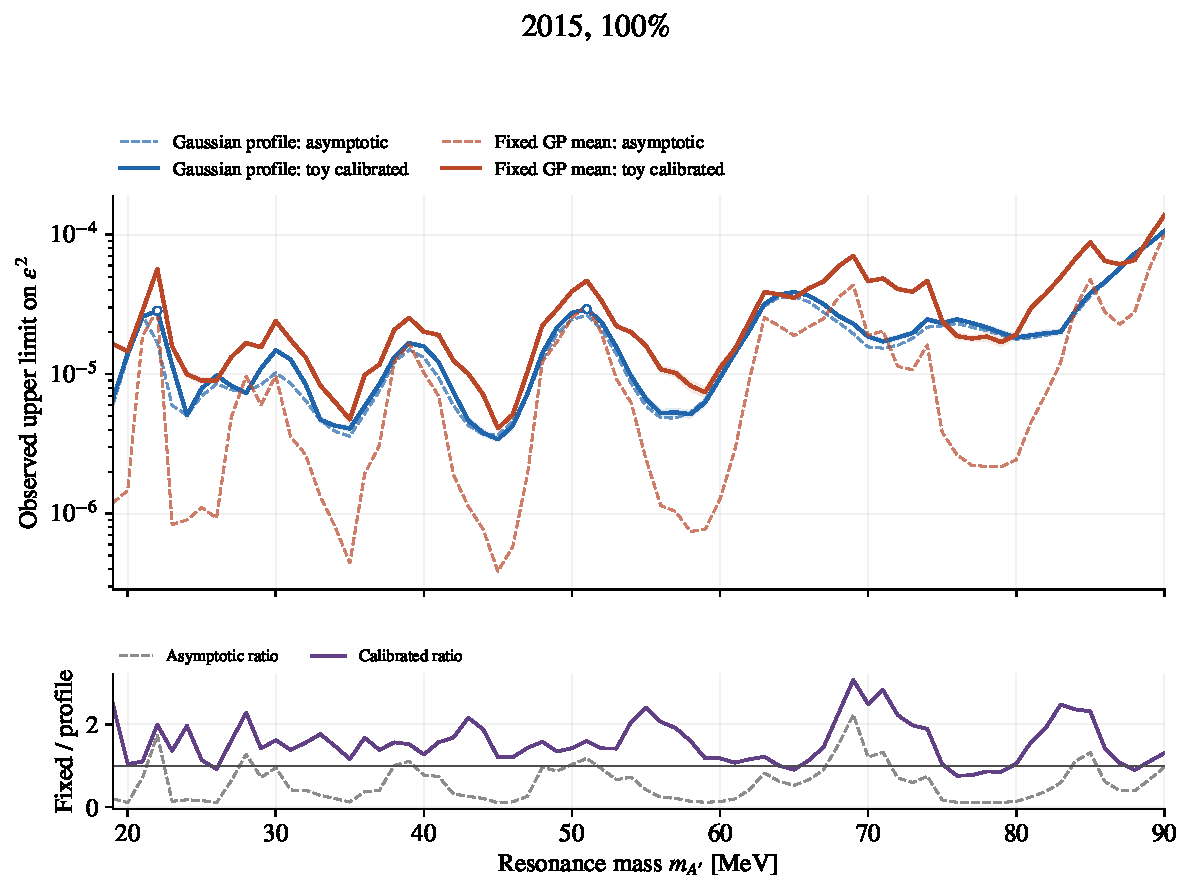
\includegraphics[width=0.96\linewidth]{../figures/v5_calibration_limits_2015.pdf}
\caption{Observed asymptotic and calibrated 90\% $CL_s$ limits for 2015
using the two background treatments. Calibration envelopes cover the two
stated generating shapes. Shading and open precision markers refer to
finite Monte Carlo accuracy; they are not expected-limit bands.}
\label{v5-fig:cal-limits-2015}
\end{figure}
\begin{figure}[htbp]\centering
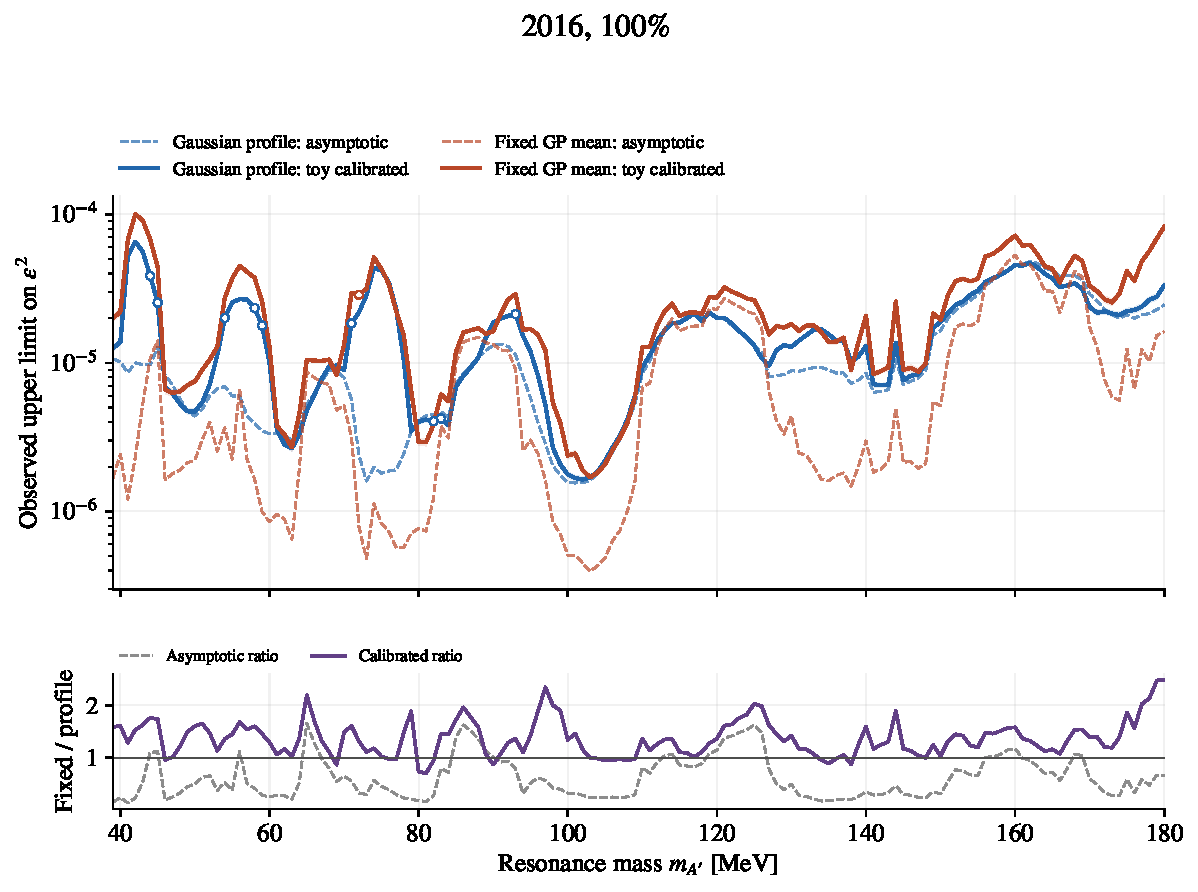
\includegraphics[width=0.96\linewidth]{../figures/v5_calibration_limits_2016.pdf}
\caption{The same comparison for full 2016. The pronounced change is
localized and depends on the archived stress construction. A resolved
calibration endpoint does not remove the source-convergence qualifications
or inherited numerical exception.}
\label{v5-fig:cal-limits-2016}
\end{figure}
\begin{figure}[htbp]\centering
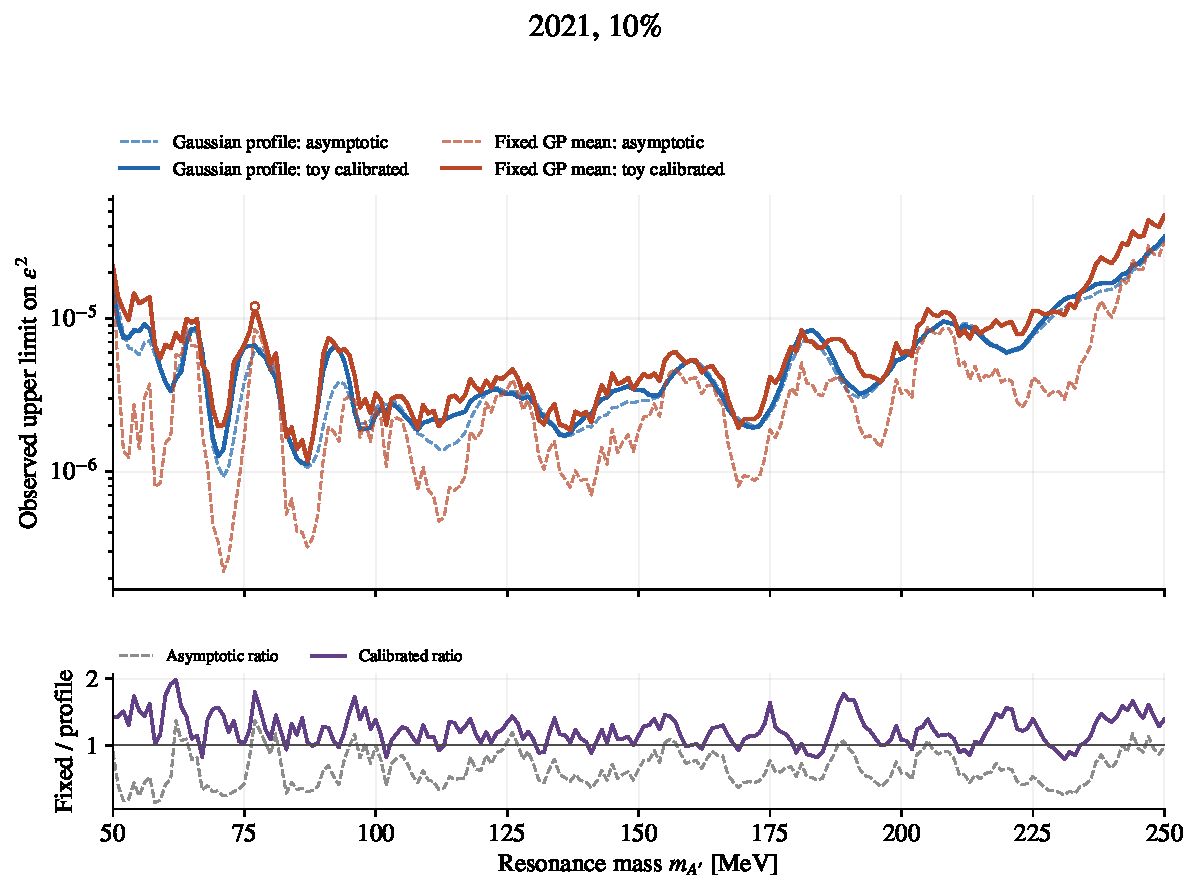
\includegraphics[width=0.96\linewidth]{../figures/v5_calibration_limits_2021.pdf}
\caption{The same comparison for native 2021 10\%. Both methods use the
same physical sample and background-truth alternatives; the observed
comparison does not measure an expected sensitivity gain.}
\label{v5-fig:cal-limits-2021}
\end{figure}
\begin{figure}[htbp]\centering
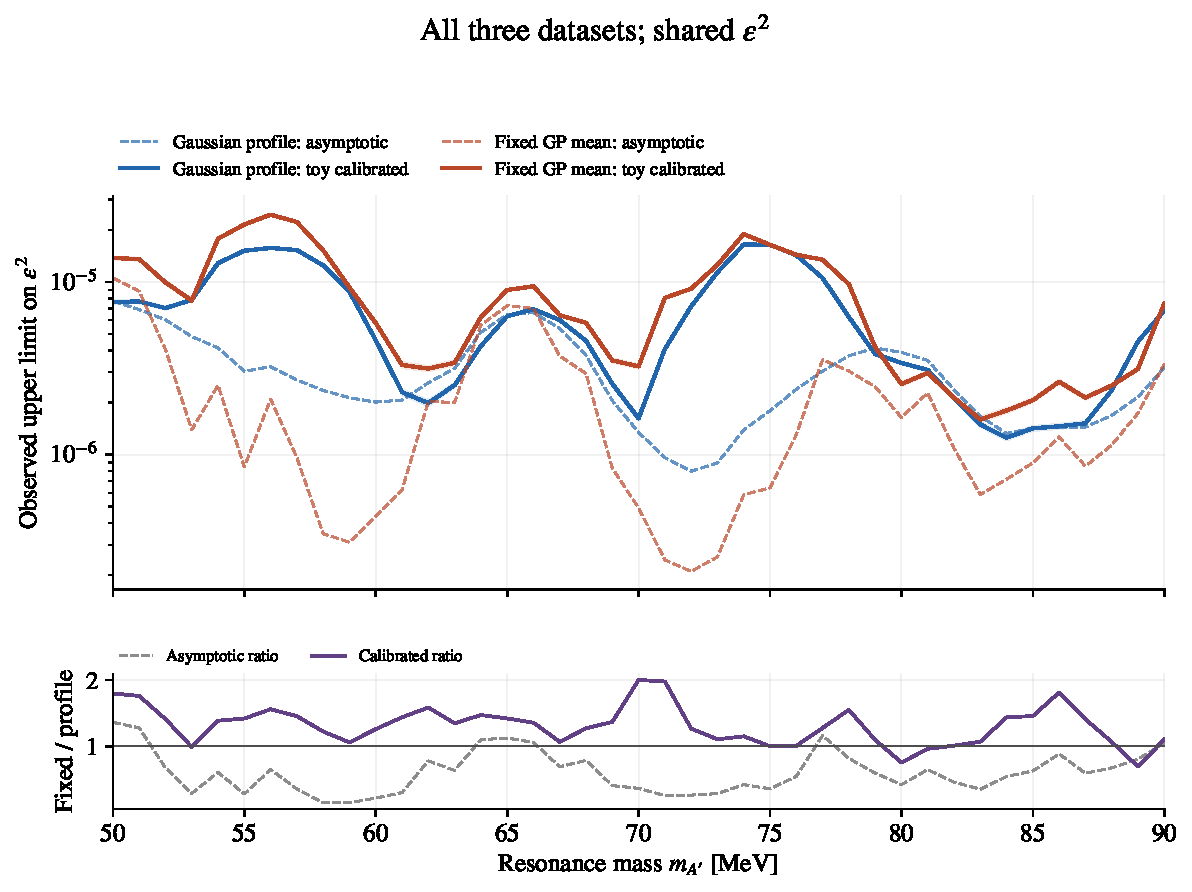
\includegraphics[width=0.96\linewidth]{../figures/v5_calibration_limits_combined.pdf}
\caption{The three-dataset common-range comparison. This calibration
covers 41 masses, rather than the later 232-mass union scan. It uses a
shared physical coupling and either all local-GP or all archived-stress
constituent backgrounds; mixed truth assignments are not included.}
\label{v5-fig:cal-limits-combined}
\end{figure}

\begin{figure}[htbp]\centering
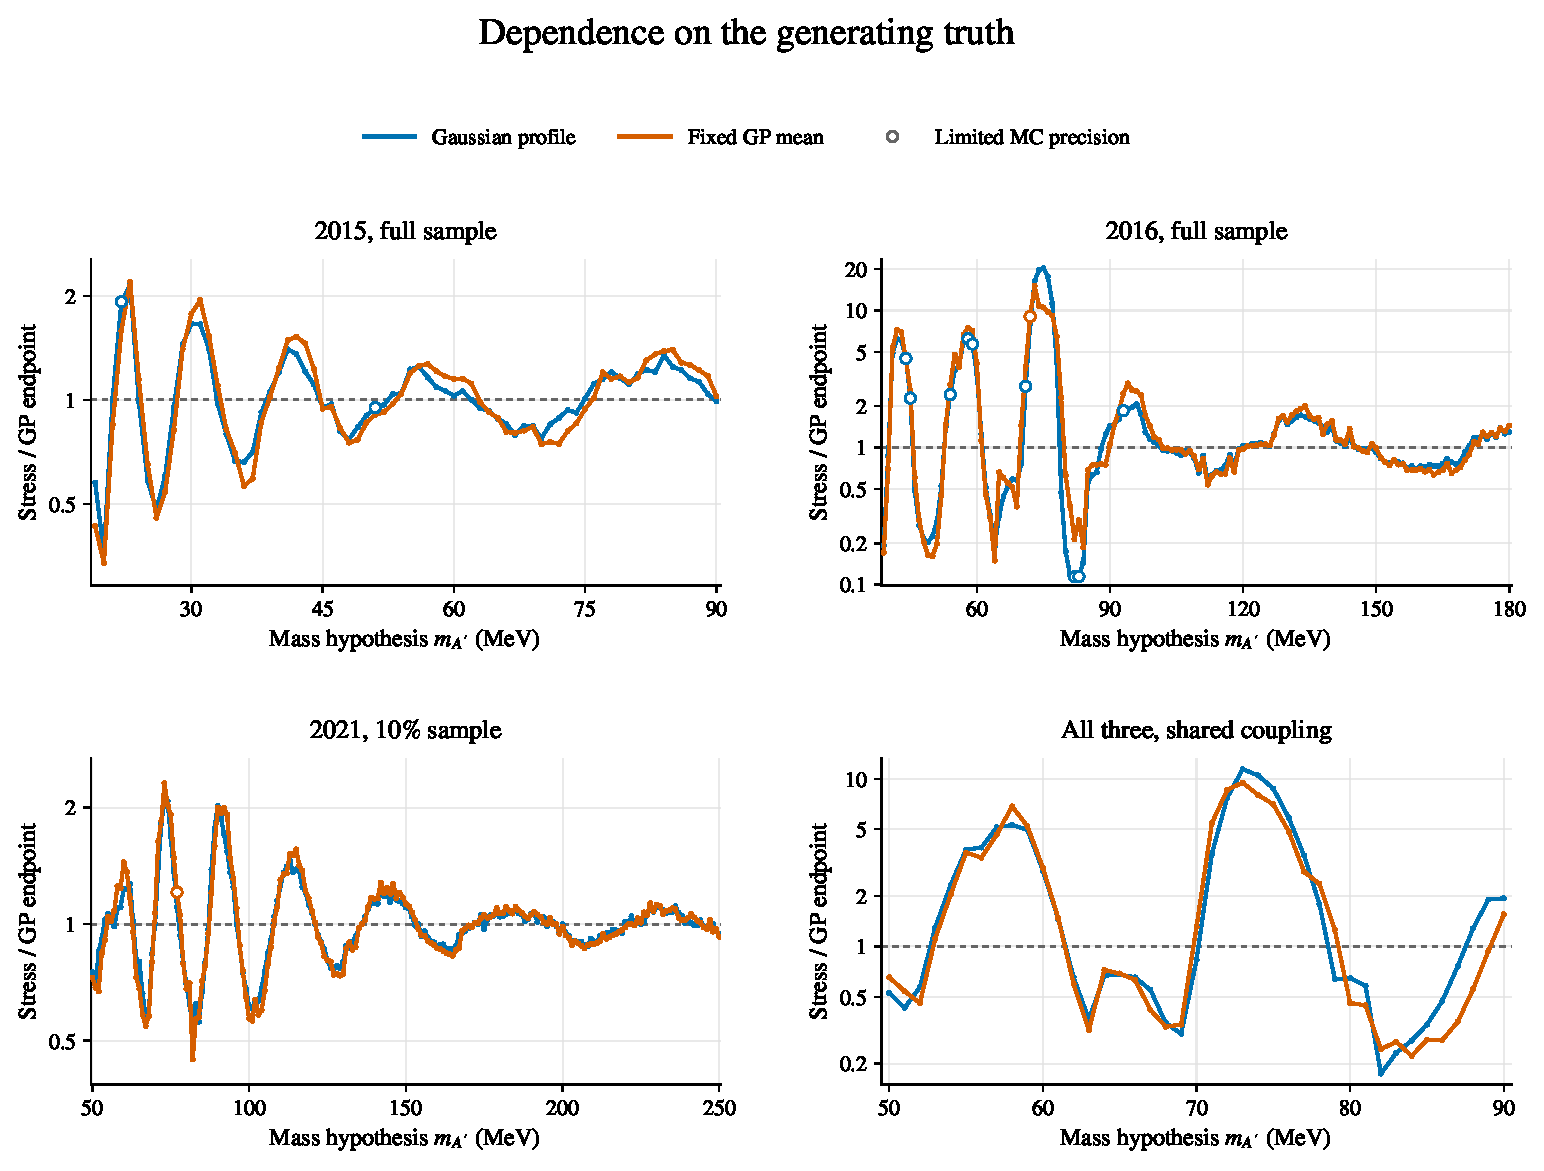
\includegraphics[width=0.96\linewidth]{../figures/v5_calibration_truth_dependence.pdf}
\caption{Ratio of the stress-truth to local-GP calibrated endpoint.
Values above one indicate that the stress background controls the larger
endpoint; values below one indicate that the local-GP control does.
Open circles mark limited precision in at least one component, and gaps
retain unavailable or censored ratios. This comparison diagnoses the
chosen background family rather than certifying either member.}
\label{v5-fig:cal-truth-dependence}
\end{figure}

At combined 66~MeV, the stress background gives a mean signed local
significance mapping of $+8.94$ with spread 0.97, while the local-GP
control gives $-0.11$ with spread 1.01. Their similar spreads and different
centers show that the effect is predominantly a shifted expected fitted
signal. All 500 stress-background-only validation spectra exceed the
observed statistic. The envelope local probability is consequently
near one. It does not identify an observed particle, and removing the
stress shape because it weakens the result would not establish a justified
background choice.

\begin{figure}[htbp]\centering
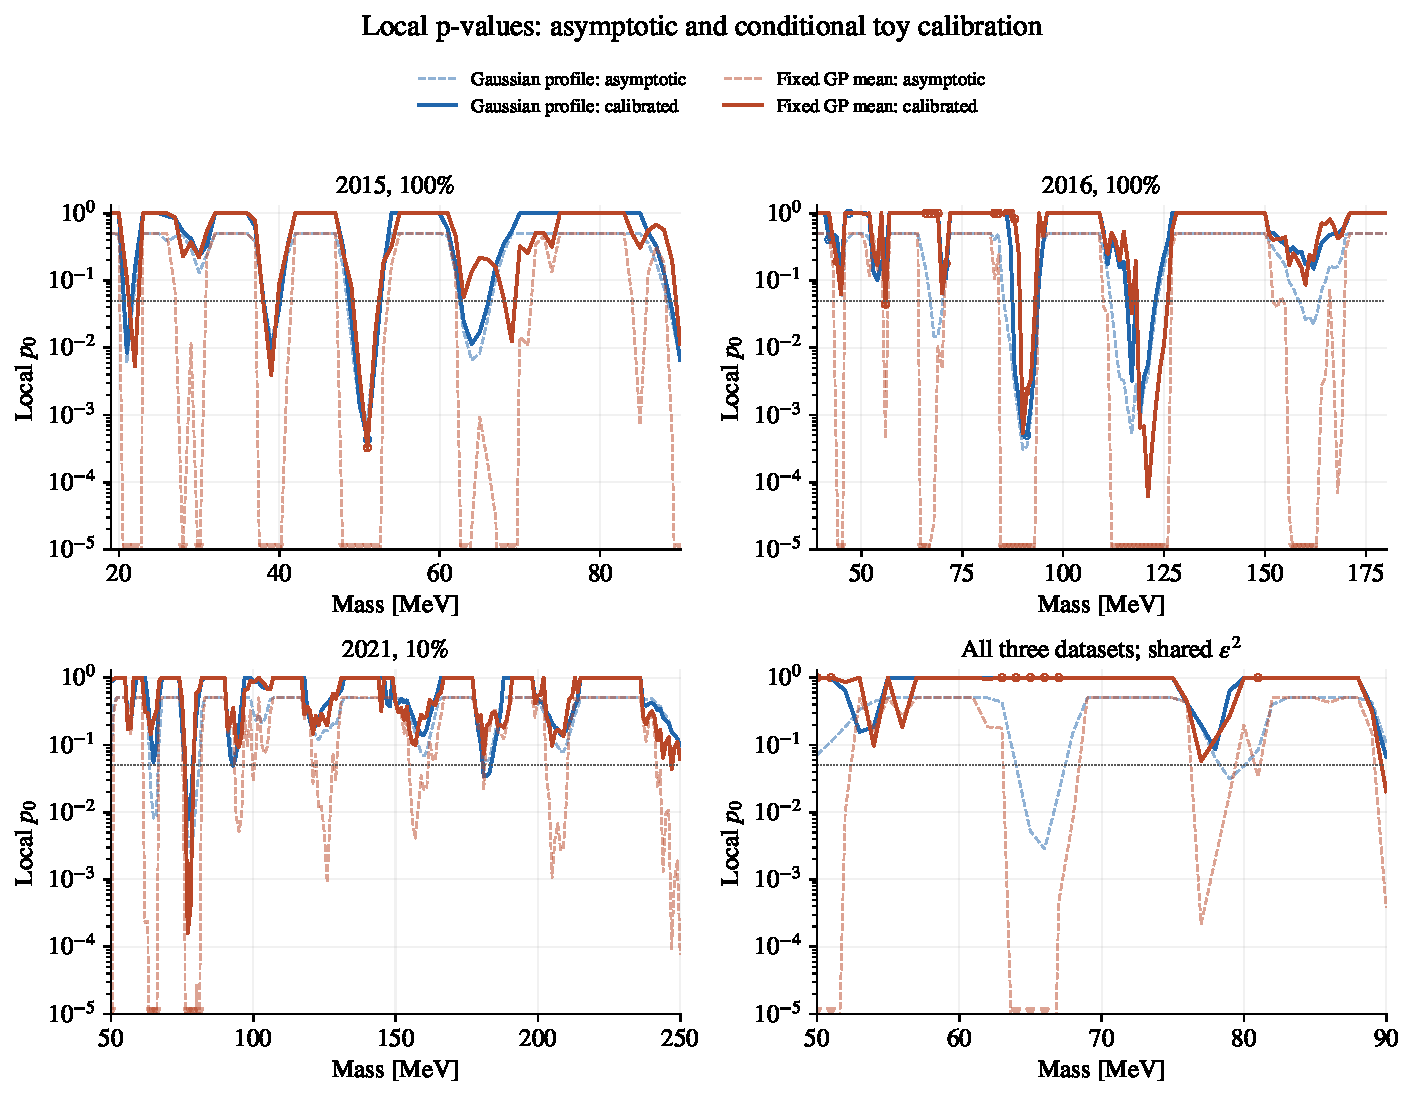
\includegraphics[width=0.96\linewidth]{../figures/v5_calibration_local_pvalues.pdf}
\caption{Asymptotic local probabilities and the larger background-only
tail from the two calibration truths. The empirical bounded-statistic
convention gives one when the discovery statistic is zero; the earlier
asymptotic display gives 0.5. Triangles retain asymptotic values below the
plotting floor. Open circles flag limited Monte Carlo precision or a
noisy estimate displayed at one; numerical ledgers retain unclipped values.
No curve in this figure includes a global trials correction.}
\label{v5-fig:cal-local-probabilities}
\end{figure}

\subsection{Interpolation offsets and a useful diagnostic}
\label{v5-sec:interpolation-offset}
An unfluctuated generating spectrum can already reveal why the fitted
signal is shifted. Train the background model on the sidebands of that
spectrum, obtaining $\bar b_t$, then compare its interpolation with the
known generating counts $b_t$ inside the gap. Project that residual onto
the signal template:
\begin{equation}
 \delta A_{\rm lin}=
 \frac{w^TV^{-1}(b_t-\bar b_t)}{w^TV^{-1}w},\qquad
 V=\operatorname{diag}(\bar b_t)+C.
 \label{v5-eq:offset-projection}
\end{equation}
The fixed-background version sets $C=0$. A positive projection means
that the smooth interpolation leaves a residual resembling a positive
signal; a negative projection means it tends to absorb one.

\begin{figure}[htbp]\centering
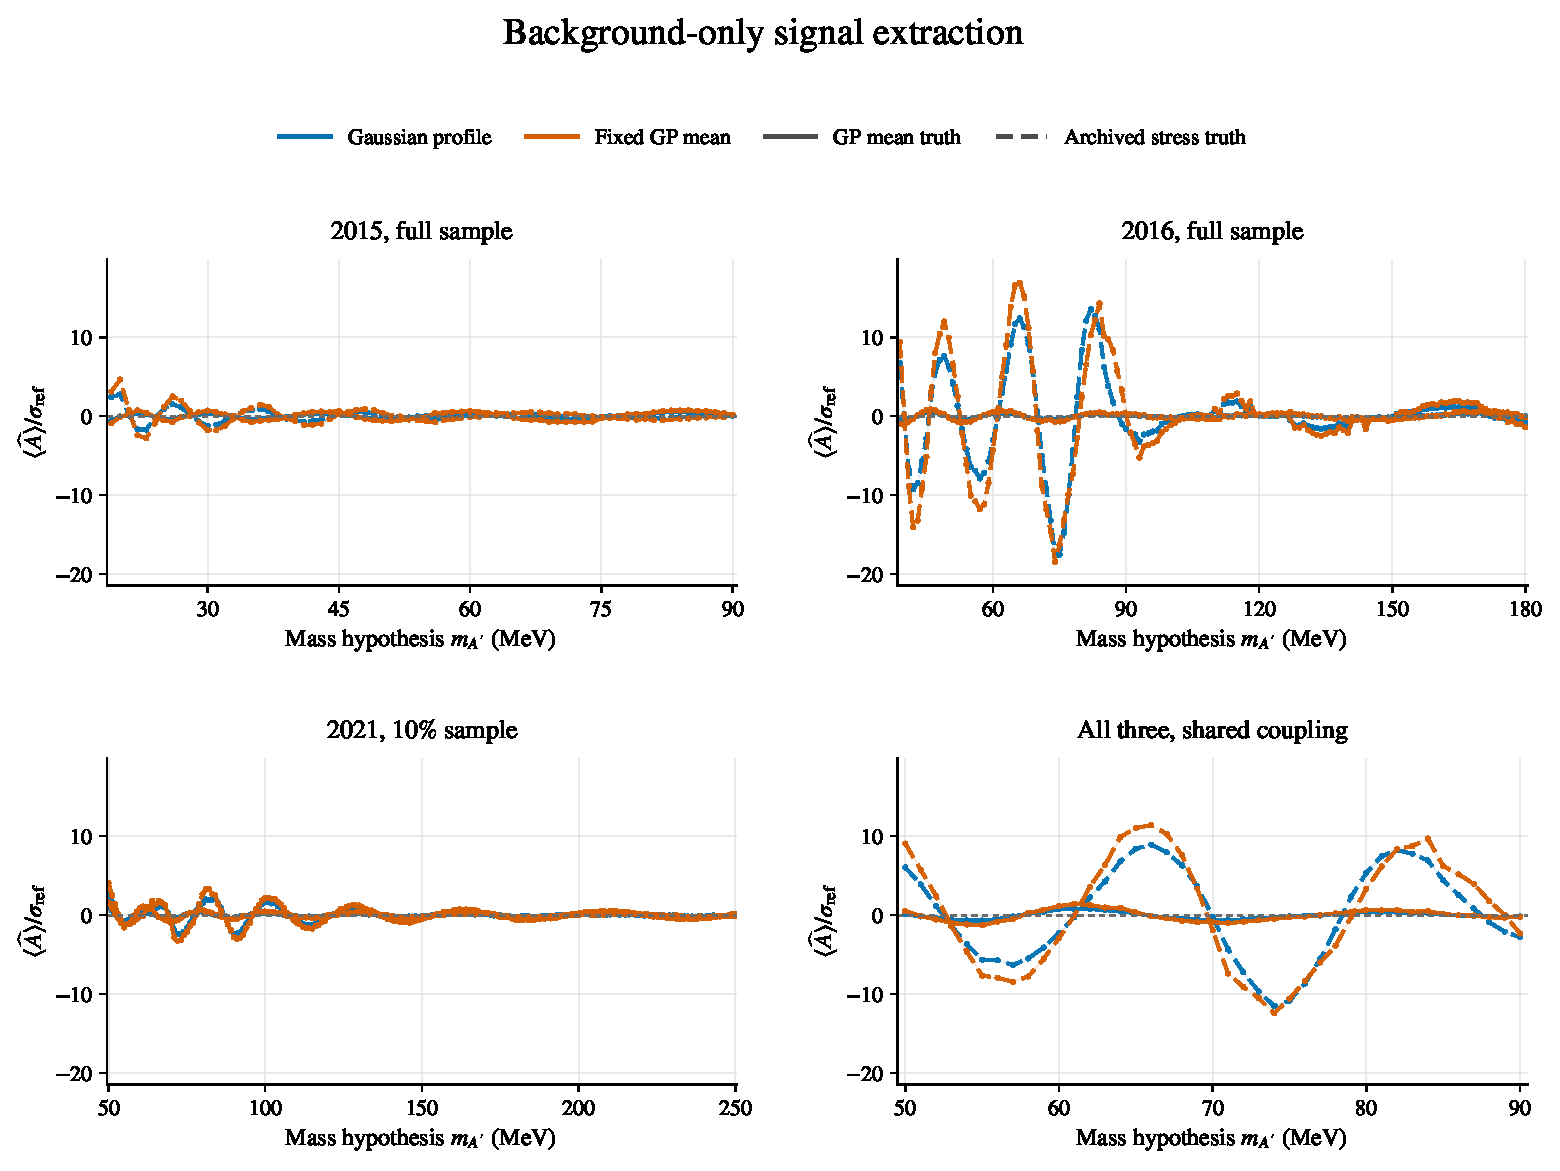
\includegraphics[width=0.96\linewidth]{../figures/v5_calibration_bias_by_truth.pdf}
\caption{Mean fitted background-only yield in units of one fixed
reference error, from 500 independently generated spectra per mass
and truth. Solid and dashed curves distinguish the two backgrounds.
Pointwise 95\% intervals describe Monte Carlo precision on each mean.
This normalization differs from a pull using each toy's random fitted
error; the plot does not measure a bias in observed data.}
\label{v5-fig:cal-mean-response}
\end{figure}

For the profiled 2016 stress ensembles, the median absolute mean offset
is 1.157 reference errors, while the median absolute discrepancy between
the ensemble mean and Eq.~\ref{v5-eq:offset-projection} is 0.031.
For the common-range combination these quantities are 5.361 and 0.035.
Thus a deterministic interpolation residual explains much of the
conditional shift without requiring random fluctuations to generate it.
This makes the projection useful for locating problematic mass regions,
comparing independently justified background shapes, and designing
paired checks of kernel policies before expensive simulations.
It is an approximation and a diagnostic, not an automatic correction
to data or a substitute for validation of the full likelihood-ratio tails.

\subsection{Independent validation in plain language}
A positive injection supplies a known answer: the true signal yield.
If a claimed 90\% upper bound falls below that yield too often, the
procedure excludes a signal that was actually present more often than
its nominal benchmark permits. The validation plot asks this question
before and after calibration on separately seeded spectra. At the true
injected yield, the envelope excludes only when both background calibrations
give $CL_s<0.10$. Each point represents one mass, one generating truth
and one method. Counts are not pooled across masses.

\begin{figure}[htbp]\centering
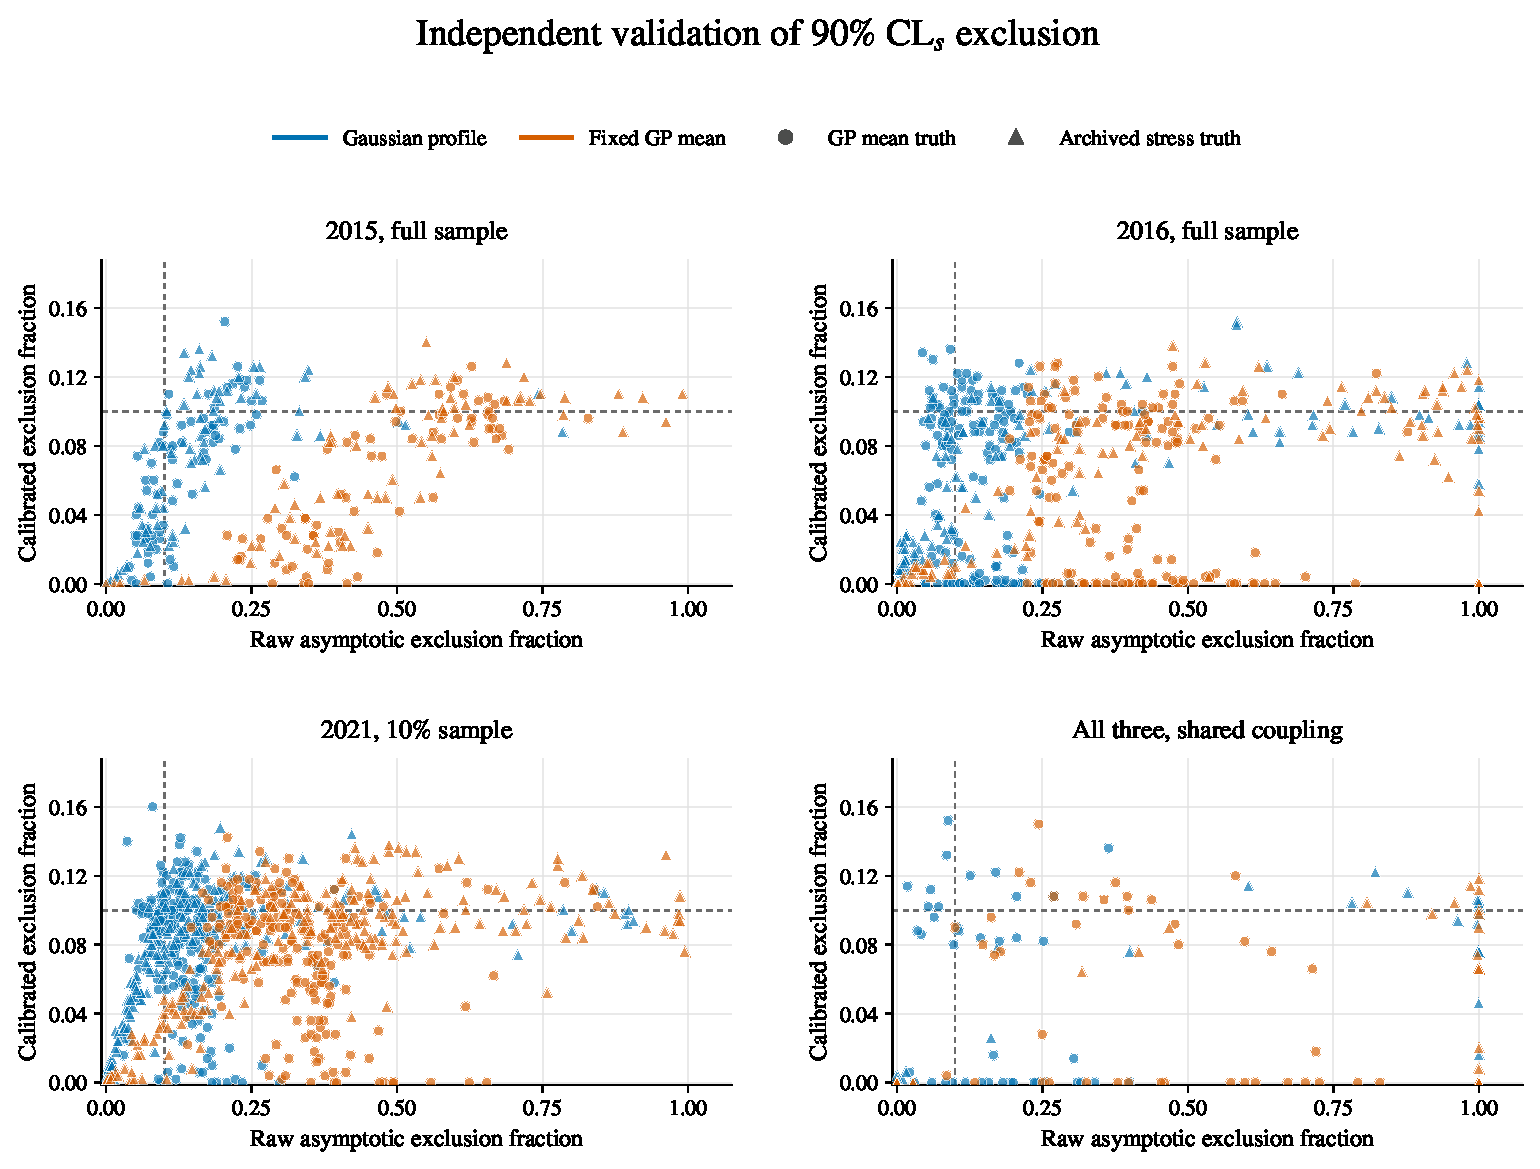
\includegraphics[width=0.96\linewidth]{../figures/v5_calibration_validation_exclusion.pdf}
\caption{Independent validation with five-reference-error injections.
The horizontal coordinate is the fraction of 500 spectra excluding the
known injected yield with the raw asymptotic rule; the vertical coordinate
uses the calibrated two-truth envelope. A point far to the right has an
excessive raw exclusion rate. A point below the horizontal 0.10 guide
indicates a conservative calibrated rate in that cell. The guides mark
the nominal benchmark, not an expected discovery probability. Finite
counts and Monte Carlo uncertainty limit the precision of each conclusion.}
\label{v5-fig:cal-validation}
\end{figure}

\begin{table}[H]\centering\small
\begin{tabular}{lrrr}\toprule
Validation family & Cells & Raw adjusted flags & Calibrated adjusted flags\\\midrule
True-yield exclusion & 3,648 & 2,039 & 0\\
Background-only local rejection & 1,824 & 952 & 0\\\bottomrule
\end{tabular}
\caption{One-sided binomial tests for rates above 10\% for true-yield
exclusion and above 5\% for local background-only rejection, with Holm
adjustment within each family at 0.05. A flag counts a failed cell-level
rate test; it is not an individual excluded toy. The full table includes
both background treatments and both truths.}
\label{v5-tab:cal-validation}
\end{table}

Even the profiled method has raw excess-rate flags: the GP and stress
truths give respectively 179/912 and 326/912 flagged exclusion cells,
and 50/456 and 140/456 flagged local-rejection cells. These results
prevent a claim that large event counts or small historical mean pulls
alone establish an adequate asymptotic mapping over the tested family.
After calibration, no adjusted flags remain in the complete suite.
That result supports the stated conditional procedure, but the tests
have limited power. With 500 spectra per cell, the first Holm exclusion
step requires at least 81/500 exclusions, or 16.2\%, to reject the 10\%
null in this family. The analogous local-rejection step begins at
48/500, or 9.6\%, against a 5\% null. No flags therefore does not
certify percent-level accuracy at every mass.

The same background disagreement can reduce detection power. At combined
66~MeV a five-reference-error signal generated on the local-GP truth
passes the raw local $p_0<0.05$ criterion in 499/500 trials but the
calibrated criterion in 0/500. Under the stress background the
background-only raw test fires in 500/500 trials, compared with 26/500
after calibration. The conservative envelope protects against this
false-positive mechanism at a cost for signals on the other truth.
An observed-limit ratio alone cannot measure that tradeoff; a fair power
comparison needs fixed physical signals and comparable error control.

\subsection{The targeted 71 MeV follow-up and remaining qualification}
The reverse-injection smooth truth that produced the 71~MeV failure is
not included among the two calibration truths. A retrospective check
replayed its original 1,500 spectra, 500 at each of zero, two and five
reference errors, with dense GP refits and the full conditioned covariance.
At the stronger injection the calibrated true-yield exclusion point
estimates are 3/500 for the profile and 2/500 for the fixed mean, compared
with their raw values of 145/500 and 349/500. This is conservative behavior
under that selected truth. However, 682 of the 3,000 method--toy decisions
have limited calibration Monte Carlo precision. These reused spectra
supply an auxiliary diagnosis, not a new independent validation sample
or truth-independent coverage.

The remaining scientific task is to qualify a background family using
source fits, sidebands and independent or explicitly held-out predictive
controls, and then validate the complete selected analysis policy. A
poorly qualified stress model need not become a mandatory physical
possibility, but its effect cannot be dismissed solely because it weakens
a result. The inherited 2016 numerical exception must be resolved
separately. These requirements define the scope of the present unblinding
review and remain visible alongside the proposed asymptotic primary results.
